\chapter{Metodologia}

Neste capítulo, serão apresentadas as técnicas utilizadas para solução do problema. O projeto 
foi realizado em um ano e sua concepção foi dividida em três frentes, nomeadamente: desenvolvimento 
da solução para o modelo da planta com controlador simulado, controle da planta simulada com o 
controlador implementado em dispositivo físico (microcontrolador) e a implementação final em dispositivo real. 
As etapas pormenorizadas do projeto são as seguintes:

\begin{enumerate}
 \item Desenvolvimento da solução para o modelo da planta com controlador simulado
  \begin{enumerate}
    \item Definição e modelagem da planta de estudo;
    \item Construção do ambiente de simulação;
    \item Validação do modelo;
    \item Implementação e validação da estratégia de controle.
  \end{enumerate}
 \item Controle da planta simulada com o controlador em dispositivo físico
  \begin{enumerate}
    \item Discretização da planta de estudo seguido da obtenção da sua equação de diferenças;
    \item Discretização do controlador seguido da obtenção da sua equação de diferenças;
    \item Configuração do ambiente de testes com a planta rodando no computador, e o 
    controlador rodando no microcontrolador (comunicação UART).
  \end{enumerate}
  \item Implementação em dispositivo real
  \begin{enumerate}
    \item Configuração do ambiente com a planta real e o microcontrolador (comunicação UART);
    \item Implementação da estratégia de controle no microcontrolador;
    \item Testes de validação da estratégia de controle na planta física.
  \end{enumerate}
\end{enumerate}

\section{Desenvolvimento da solução para o modelo da planta}
\markright{\thesection ~~~ Metodologia}
\label{metodo}

A modelagem dos manipuladores robóticos visa descrever como os elos e juntas estão 
configurados fisicamente para tornar possível a configuração de sua orientação e sua posição 
\cite{paul1981robot}. Com isso, ao passar uma trajetória de referência que a 
ferramenta de trabalho deve descrever, as demais juntas se reajustam de modo a garantir 
que a ferramenta sempre esteja corretamente posicionada. A estratégia de controle deve, 
então, estar adequadamente sintonizada para garantir o seguimento acurado da trajetória.

No presente trabalho são realizadas duas modelagens para o manipulador: a modelagem 
cinemática e a modelagem dinâmica. A modelagem cinemática visa descrever a amplitude 
de movimento das juntas robóticas, ao passo que a modelagem dinâmica busca considerar 
as forças e torques que produzem o movimento, descrevendo, explicitamente, a relação 
entre força e movimento \cite{Spong}.

A principal ferramenta utilizada para se obter o modelo cinemático direto de um 
manipulador robótico é a convenção de \textit{Denavit-Hartenberg} (DH) \cite{paul1981robot}
. A modelagem dinâmica, por sua vez, pode ser realizada por meio das equações de 
textit{Euler-Lagrange}, que correspondem a um método baseado na energia do sistema 
\cite{Park}.

\subsection{Convenção de \textit{Denavit-Hartenberg}}
\markright{\thesubsection ~~~ Convenção de \textit{Denavit-Hartenberg}}
\label{DH}

Considera-se que o manipulador a ser modelado é de cadeia aberta, ou seja, um manipulador 
que o número de graus de liberdade seja igual ao número de articulações ativas.
Além disso, ele deve ser constituído por $n+1$ elos conectados por $n$ juntas, onde 
o elo $0$ é convencionalmente fixado ao solo. Assim sendo, segundo \citeonline{siciliano}, 
a equação cinemática direta para o manipulador pode ser calculada a partir de:

\begin{equation}
  \begin{gathered}
    T^0_n = A^0_1(q_1)A^1_2(q_2)\cdots A^{n-1}_n(q_n)
  \end{gathered}
  \label{eq:cinematicaDireta}
\end{equation}

A relação \eqref{eq:cinematicaDireta} se refere à transformação de coordenadas descrevendo 
a posição e a orientação do eixo $n$ em relação à base (eixo $0$) \cite{siciliano}. Segundo
\citeonline{Spong}, na convenção DH, cada transformação homogênea $A_i$ representada em
\eqref{eq:cinematicaDireta} equivale ao produto de quatro transformações básicas, apresentado a seguir:

\begin{equation*}
  \begin{gathered}
    A_i = Rot_{z,\theta_i}Trans_{z,\theta_i}Trans_{x,\alpha_i}Rot_{x,\alpha_i} \\[0.5cm]
    =\begin{bmatrix}
     \cos(\theta_i) & -\sin(\theta_i) & 0 & 0 \\
     \sin(\theta_i) & \cos(\theta_i) & 0 & 0 \\
     0 & 0 & 1 & 0 \\
     0 & 0 & 0 & 1 \\
    \end{bmatrix}
    \begin{bmatrix}
     1 & 0 & 0 & 0 \\
     0 & 1 & 0 & 0 \\
     0 & 0 & 1 & d_i \\
     0 & 0 & 0 & 1 \\
    \end{bmatrix} \\
    \times \begin{bmatrix}
     1 & 0 & 0 & a_i \\
     0 & 1 & 0 & 0 \\
     0 & 0 & 1 & 0 \\
     0 & 0 & 0 & 1 \\
    \end{bmatrix}
    \begin{bmatrix}
     1 & 0 & 0 & 0 \\
     0 & \cos(\alpha_i) & -\sin(\alpha_i) & 0 \\
     0 & \sin(\alpha_i) & \cos(\alpha_i) & d_i \\
     0 & 0 & 0 & 1 \\
    \end{bmatrix} \\
  \end{gathered}
\end{equation*}
\begin{equation}
  \begin{gathered}
    =
    \begin{bmatrix}
     \cos(\theta_i) & -\sin(\theta_i)\cos(\alpha_i) & \sin(\theta_i)\sin(\alpha_i) & a_i\cos(\theta_i) \\
     \sin(\theta_i) & \cos(\theta_i)\cos(\alpha_i) & -\cos(\theta_i)\sin(\alpha_i) & a_i\sin(\theta_i) \\
     0 & \sin(\alpha_i) & \cos(\alpha_i) & d_i \\
     0 & 0 & 0 & 1 \\
    \end{bmatrix}
  \end{gathered}
  \label{eq:matTransHomog}
\end{equation}

A matriz final encontrada em \eqref{eq:matTransHomog} é chamada de Matriz de
Trasformação Homogênea. Os quatro parâmetros da relação \eqref{eq:matTransHomog} 
representam: tamanho do elo ($a_i$), deslocamento do elo ($d_i$), 
giro do elo ($\alpha_i$), ângulo da junta ($\theta_i$). De acordo com 
\citeonline{paul1981robot}, os parâmetros são obtidos através do procedimento a seguir:

\begin{itemize}
  \item Rotacionar $x_i$ em torno do eixo $z_{i}$ um ângulo $\theta_i$;
  \item Transladar ao longo do eixo $z_{i}$ uma distância $d_i$;
  \item Transladar ao longo de $x_{i+1}$ uma distância $a_i$; 
  \item Rotacionar $z_i$ em torno de $x_{i+1}$ o ângulo de torção $\alpha_i$
\end{itemize}

Assim sendo, a modelagem cinemática é obtida através da multiplicação de diversas
matrizes de transformação homogêneas individuais, conforme
\eqref{eq:cinematicaDireta}. Com isso, para um manipulador com três graus de 
liberdade, a transformação de coordenadas do elemento terminal em relação a base é
dada por $T^0_3=A_1A_2A_3$ .

\subsubsection{Cinemática Diferencial e o Jacobiano}

A cinemática diferencial é responsável por fornecer a relação entre as velocidades das juntas
e a correspondente velocidade final linear e angular da ferramenta de trabalho \cite{siciliano}. Essa 
relação é descrita por uma matriz denominada jacobiana geométrica, que depende da configuração do manipulador. 
O Jacobiano Analítico, por outro lado, é expresso por meio da diferenciação da função cinemática direta com 
relação às variáveis das juntas. A obtenção da matriz Jacobiana é fundamental para determinar as equações 
de movimento do manipulador robótico.

Segundo \citeonline{Spong}, considerando um manipulador com \textit{n} graus de liberdade, a equação da cinemática direta 
pode ser escrita na forma:

\begin{equation}
  \begin{gathered}
    T^{0}_n(q) = \begin{bmatrix}
     R^{0}_n(q) & o^{0}_n(q)\\
     0 & 1\\
    \end{bmatrix}
  \end{gathered}
  \label{eq:cinematicaDireta_2}
\end{equation}

A equação \eqref{eq:cinematicaDireta_2} é a mesma que \eqref{eq:cinematicaDireta}, onde $q = [q_1,...,q_n]^T$ é o vetor das 
variáveis das juntas, $R^{0}_n(q)$ a matriz de rotação, $o^{0}_n(q)$ o vetor de translação, $0$ a perspectiva e $1$ o 
fator de escala. As relações da velocidade linear $v^0_n$ e a velocidade angular $\omega^0_n$ em função das velocidades 
das juntas é linear \cite{siciliano} e pode ser expressa por:

\begin{equation}
  \begin{gathered}
    v^0_n = J_v \dot{q}
  \end{gathered}
  \label{eq:jacob_velLinar}
\end{equation}

\begin{equation}
  \begin{gathered}
    \omega^0_n = J_\omega \dot{q}
  \end{gathered}
  \label{eq:jacob_velAngular}
\end{equation}
onde $J_v$ e $J_\omega$ são matrizes $3 \times n$. É possível ainda, reescrever \eqref{eq:jacob_velLinar} e
\eqref{eq:jacob_velAngular} da seguinte forma:
\begin{equation}
  \begin{gathered}
    \zeta = J\dot{q}
  \end{gathered}
  \label{eq:jacob_ambos}
\end{equation}

\begin{equation}
  \begin{gathered}
    \zeta = \begin{bmatrix}
     v^0_n\\
     \omega^0_n\\
    \end{bmatrix}
    \quad \textrm{e} \quad 
    J = \begin{bmatrix}
     J_v\\
     J_\omega\\
    \end{bmatrix}
  \end{gathered}
\end{equation}

O vetor $\zeta$ também pode ser chamado de velocidade do corpo \cite{Spong} e é importante notar que
ele não é a derivada de uma variável de posição. A matriz $J$ é chamado de \textbf{Jacobiano} e trata-se
de uma matriz $6 \times n$ .

Combinando as partes angular e linear, segundo \citeonline{siciliano}, a metade de cima da matriz do Jacobiano é
dada por:

\begin{equation}
  \begin{gathered}
    J_{v_i} = 
      \left\{
	\begin{array}{cl}
	  z_{i-1} \times (o_n - o_{i-1}) & \text{para a $i$-ésima junta revoluta}\\
	  z_{i-1} 			 & \text{para a $i$-ésima junta prismática}
	\end{array}
      \right.
  \end{gathered}
\end{equation}

A segunda metade, ou a metade baixo da matriz do Jacobiano é dada por:

\begin{equation}
  \begin{gathered}
    J_{\omega_i} = 
      \left\{
	\begin{array}{cl}
	  z_{i-1} & \text{para a $i$-ésima junta revoluta}\\
	  0 	  & \text{para a $i$-ésima junta prismática}
	\end{array}
      \right.
  \end{gathered}
\end{equation}

Juntando ambas as metades da matriz do Jacobiano obtém-se para a junta revoluta a equação \eqref{eq:revolJacobiano}
e para a junta prismática \eqref{eq:prismaticJacobiano}:

\begin{equation}
  \begin{gathered}
    J_i = \begin{bmatrix}
     z_{i-1} \times (o_n - o_{i-1})\\
     z_{i-1}\\
    \end{bmatrix}
  \end{gathered}
  \label{eq:revolJacobiano}
\end{equation}

\begin{equation}
  \begin{gathered}
    J_i = \begin{bmatrix}
     z_{i-1}\\
     0\\
    \end{bmatrix}
  \end{gathered}
  \label{eq:prismaticJacobiano}
\end{equation}

Assim sendo, as únicas ferramentas necessárias para calcular o Jacobiano são os 
vetores unitários $z_i$ e as coordenadas das origens $o_1, ..., o_n$. As coordenadas
para $z_i$ são dadas pelos três primeiros elementos da terceira coluna de $T^0_i$, 
enquanto as coordenadas de $o_n$ são dadas pelos três primeiros elementos da quarta
coluna de $T^0_i$ . Dessa forma, apenas a terceira e a quarta colunas da matriz de 
homogeneidade $T$ são necessárias para obter o Jacobiano. \cite{Spong}

\subsection{Equações de \textit{Euler-Lagrange}}
\markright{\thesubsection ~~~ Equações de \textit{Euler-Lagrange}}
\label{EL}

Com o conjunto de coordenadas generalizadas independentes $q_j$, $j = 1, \dotsc, n$, onde $n$ 
representa os graus de liberdade do manipulador, o Lagrangiano do sistema 
é definido pela relação \eqref{eq:lagrangiano} \cite{Spong}, onde $K$ representa 
a energia cinética e $P$ a energia potencial do sistema:

\begin{equation}
  \begin{gathered}
    L = K - P
  \end{gathered}
  \label{eq:lagrangiano}
\end{equation}

Segundo \citeonline{Spong}, em geral, as equações de \textit{Euler-Lagrange}
aplicadas a um sistema de $n$ coordenadas podem ser representadas na forma da
Equação \eqref{eq:EL}, onde a força generalizada $\tau_i$ representa as forças 
externas e torques não deriváveis de uma função potencial:

\begin{equation}
  \begin{gathered}
    \frac{d}{dt}\frac{\partial L}{\partial \dot q_i}-\frac{\partial L}{\partial q_i} = \tau_i
  \end{gathered}
  \label{eq:EL}
\end{equation}

Conforme apresentado, as equações de \textit{Euler-Lagrange} podem ser 
usadas para derivar as equações dinâmicas de maneira direta. É possível computar 
esses termos para um manipulador robótico de $n$ elos por meio das fórmulas da 
energia cinética e da energia potencial usando as variáveis de articulação obtidas a partir da modelagem 
de \textit{Denavit-Hartenberg} como coordenadas generalizadas \cite{Spong}.

\subsubsection{Energia cinética para um manipulador de $n$ elos}

Segundo \citeonline{Spong} a energia cinética é dada pela soma de dois 
termos: a energia de translação, obtida concentrando toda a massa do objeto no 
centro de massa, e a energia cinética rotacional em torno do centro de massa. 
Assim, a energia cinética do manipulador é dada por:

\begin{equation}
  \begin{gathered}
    K=\frac{1}{2}mv^Tv+\frac{1}{2}\omega^T\Gamma \omega
  \end{gathered}
  \label{eq:energiaCinetica}
\end{equation}
onde $m$ é a massa do objeto, $v$ e $\omega$ são os vetores de velocidade 
linear e angular, respectivamente, e $\Gamma$ é uma matriz simétrica $3 \times 3$ 
chamada Tensor de Inércia. O Tensor de Inércia é relacionado ao quadro de 
referência inercial do manipulador. Dessa forma, é possível 
relacionar o tensor de inércia com a matriz de rotação através de uma 
transformação de similaridade:

\begin{equation}
  \begin{gathered}
    \Gamma = RIR^T
  \end{gathered}
  \label{eq:ts}
\end{equation}
onde $R$ é a matriz de rotação $R^{0}_n(q)$ obtida em \eqref{eq:jacob_velLinar}, e 
$I$ é uma matriz que não depende do movimento do objeto. 
Cada elemento dessa matriz é calculado através de integrais sobre as
regiões do espaço ocupados por todas as partes do corpo rígido:

\begin{equation}
  \begin{gathered}
    I = \begin{bmatrix}
     I_{xx} & I_{xy} & I_{xz}\\
     I_{yx} & I_{yy} & I_{yz}\\
     I_{zx} & I_{zy} & I_{zz}\\
    \end{bmatrix}
  \end{gathered}
\end{equation}

\begin{equation}
  \begin{gathered}
    I_{xx} = \iiint(y^2+z^2)\rho(x,y,z)dxdydz\\
    I_{yy} = \iiint(x^2+z^2)\rho(x,y,z)dxdydz\\
    I_{zz} = \iiint(x^2+y^2)\rho(x,y,z)dxdydz\\
    I_{xy} = I_{yx} = - \iiint xy\rho(x,y,z)dxdydz\\
    I_{xz} = I_{zx} = - \iiint xz\rho(x,y,z)dxdydz\\
    I_{yz} = I_{zy} = - \iiint yz\rho(x,y,z)dxdydz\\
  \end{gathered}
\end{equation}

Através do Tensor de Inércia, do jacobiano, da matriz de rotação e da massa de
cada parte do braço obtém-se a energia cinética do manipulador:

\begin{equation}
  \begin{gathered}
    K=\frac{1}{2}\dot q^T D(q)\dot q
  \end{gathered}
  \label{eq:ecMat}
\end{equation}
sendo:
\begin{equation}
  \begin{gathered}
    D(q)= \sum^n_{i=1}[m_iJ_{vi}(q)^TJ_{vi}(q)+J_{\omega i}(q)^TR_i(q)I_i(q)R_i(q)^TJ_{\omega i}(q)]
  \end{gathered}
  \label{eq:dq}
\end{equation}

\subsubsection{Energia potencial para um manipulador de $n$ elos}

A energia potencial do manipulador de $n$ elos é dada pela soma da energia
potencial individual de cada parte envolvida. A única fonte de energia potencial
do manipulador é a gravidade, assumindo que a massa total de cada elemento 
do manipulador está concentrada no seu centro de massa.

Segundo \citeonline{Spong}, a energia potencial é uma função apenas das 
coordenadas generalizadas e não de suas derivadas, assim, a energia 
potencial depende da configuração do robô e independe da velocidade:

\begin{equation}
  \begin{gathered}
    P = \sum^n_{i=1}P_i = \sum^n_{i=1}g^Tr_{ci}m_i
  \end{gathered}
  \label{eq:enePotencial}
\end{equation}
onde $g$ é o vetor que dá a direção da gravidade no referencial inercial, e 
$r_{ci}$ fornece as coordenadas do centro de massa do elo $i$. Sendo assim,
a matriz da energia potencial é dada por:

\begin{equation}
  \begin{gathered}
    g(q)=\phi_k=\frac{\partial P}{\partial q_k}
  \end{gathered}
  \label{eq:enePotencialMat}
\end{equation}

\subsubsection{Equações de movimento}

Aplicando o que foi exposto anteriormente, as equações de \textit{Euler-Lagrange} 
\eqref{eq:EL} podem ser expressas segundo:

\begin{equation}
  \begin{gathered}
    \sum_i d_{kj}(q)\ddot q_j + \sum_{i,j}c_{ijk}(q)\dot q_i\dot q_j + \phi_k = \tau_k \quad, \quad k=1,\dots,n
  \end{gathered}
  \label{eq:EL_Final}
\end{equation}
ou na forma matricial:
\begin{equation}
  \begin{gathered}
    D(q)\ddot q + C(q,\dot q)\dot q + g(q) = \tau
  \end{gathered}
  \label{eq:EL_FinalMat}
\end{equation}
onde $D(q)$ e $g(q)$ representam as matrizes da energia cinética e potencial, 
respectivamente, e $C(q,\dot q)$ representa uma matriz construída com os chamados
Símbolos de Christoffel, definidos matematicamente por \citeonline{Spong} através
da equação:

\begin{equation}
  \begin{gathered}
    c_{ijk} = \frac{1}{2} \left\{ \frac{\partial d_{kj}}{\partial q_i}+\frac{\partial d_{ki}}{\partial q_j}-\frac{\partial d_{ij}}{\partial q_k} \right\}
  \end{gathered}
  \label{eq:christoffel}
\end{equation}

Como o manipulador RRR possui três juntas revolutas, e cada junta revoluta é descrita por uma matriz 
$3 \times 3$, serão necessários 27 Símbolos de Christoffel diferentes.

\section{Ensaio em malha aberta para a obtenção do modelo da planta}

O modelo matemático de um sistema é definido como um conjunto de equações que representa a sua dinâmica \cite{Ogata}. 
Esses modelos são sempre idealizações do comportamento
real e são válidos para excitações dentro de certos limites de amplitude e frequência \cite{Castrucci}.

Uma das formas de se obter o modelo de um determinado sistema $G(s)$, dentro de certos limites de amplitude e frequência,
é através dos seus dados de entrada $U(s)$ e saída $Y(s)$, vide \autoref{fig:diagEnsaioMA}. Ao aplicar na entrada uma 
referência conveniente (degrau, impulso, senoide), ignorando os fenômenos internos, obtém-se uma determinada saída que ao 
ser avaliada ao longo do tempo, ficam aparentes os parâmetros das equações diferenciais procuradas \cite{Castrucci}.

\begin{figure}[ht]
  \centering
  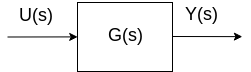
\includegraphics[width = 0.4\columnwidth]{Imagens/diagEnsaioMA.png}
  \caption{Diagrama do ensaio em malha aberta}
  \fonte{Do autor}
  \label{fig:diagEnsaioMA} 
\end{figure}

A resposta temporal de um sistema de controle é composto da resposta transitória, aquela que compreende o tempo entre o 
estado inicial e o final, e a resposta estacionária que corresponde ao comportamento do sinal de saída quando $t$
tende ao infinito \cite{Ogata}. Dependendo do comportamento das respostas do sistema, ele pode ser classificado
como de primeira ordem \eqref{eq:sistemaPrimeiraOrdem}, de segunda ordem \eqref{eq:sistemaSegundaOrdem} ou como sistema 
de ordem superior.

\begin{equation}
  \begin{gathered}
    \frac{Y(s)}{U(s)} = \frac{1}{\tau s + 1}
  \end{gathered}
  \label{eq:sistemaPrimeiraOrdem}
\end{equation}

\begin{equation}
  \begin{gathered}
    \frac{Y(s)}{U(s)} = \frac{\omega_n^2}{s^2 + 2\xi \omega_n s + \omega_n^2}
  \end{gathered}
  \label{eq:sistemaSegundaOrdem}
\end{equation}
onde:

\begin{itemize}
 \item $\tau$: constante de tempo do sistema ($\tau > 0$);
 \item $\omega_n$: frequência natural não amortecida ($\omega_n > 0$);
 \item $\xi$: coeficiente de amortecimento.
\end{itemize}

A constante de tempo do sistema de primeira ordem é definida como o instante em que a resposta 
do sistema atingiu 63,2\% de sua variação final \cite{Castrucci}. Por outro lado, para os sistemas de
segunda ordem, o que define o $\xi$ é o sobressinal máximo do sistema, e o $\omega_n$ pode ser definido
pelas constantes de tempo do sistema de segunda ordem, como por exemplo o tempo de 
acomodação. O tempo de acomodação para uma faixa de $\pm$ 2\% em torno do valor final é dado 
por \eqref{eq:tempoAcomodacao}:

\begin{equation}
  \begin{gathered}
    t_s \cong \frac{4}{\xi \omega_n}
  \end{gathered}
  \label{eq:tempoAcomodacao}
\end{equation}

\section{Projeto de sistemas de controle pelo método do lugar das raízes}

O lugar das raízes é um método simples que possibilita a representação gráfica das raízes da equação
característica para todos os valores do ganho, ou qualquer outro parâmetro da função de transferência
de malha aberta \cite{Ogata}. O projeto de controle pelo método do lugar das raízes é realizado através 
da adição de zeros e polos à função de transferência de malha aberta do sistema, forçando o lugar das raízes a passar 
pelos polos de malha fechada desejados.

No presente projeto, foram levantados três modelos para planta, um para cada uma das juntas (base, ombro, cotovelo).
Para cada uma delas foi projetado um controlador independe (conhecido na literatura como controle de juntas independes). Os projetos 
foram realizado através do método do lugar das raízes, com o auxílio da ferramenta \textit{sisotool} do \textit{Matlab}.

\section{Configuração do ambiente de simulação}

A partir dos modelos cinemáticos e dinâmicos obtidos, um ambiente de simulação é 
concebido na plataforma \textit{Matlab} (\autoref{fig:plantaSimulada}). Por meio desse 
ambiente, diferentes técnicas de controle podem ser sintetizadas e validadas para o manipulador estudado. 
Posteriormente, é feita a implementação da estratégia de controle sintetizada em dispositivo físico (microcontrolador),
sendo que a validação é realizada no ambiente de simulação 
desenvolvido por meio da técnica HIL, vide 
\autoref{fig:solucaoModelo}. Finalmente, a última etapa corresponde à implementação das 
estratégias de controle no manipulador robótico estudado (planta física). Como ilustrado 
na \autoref{fig:solucaoPlanta}, nessa etapa o microntrolador é conectado ao manipulador de 
forma a controlá-lo, fazendo-o seguir uma trajetória pré-especificada. Assim, verifica-se 
se, de fato, a resposta do sistema físico em malha fechada corresponde à resposta obtida 
por meio de simulação utilizando a técnica HIL.

\begin{figure}[h!]
  
  \centering
  \begin{subfigure}{.5\textwidth}
    \centering
    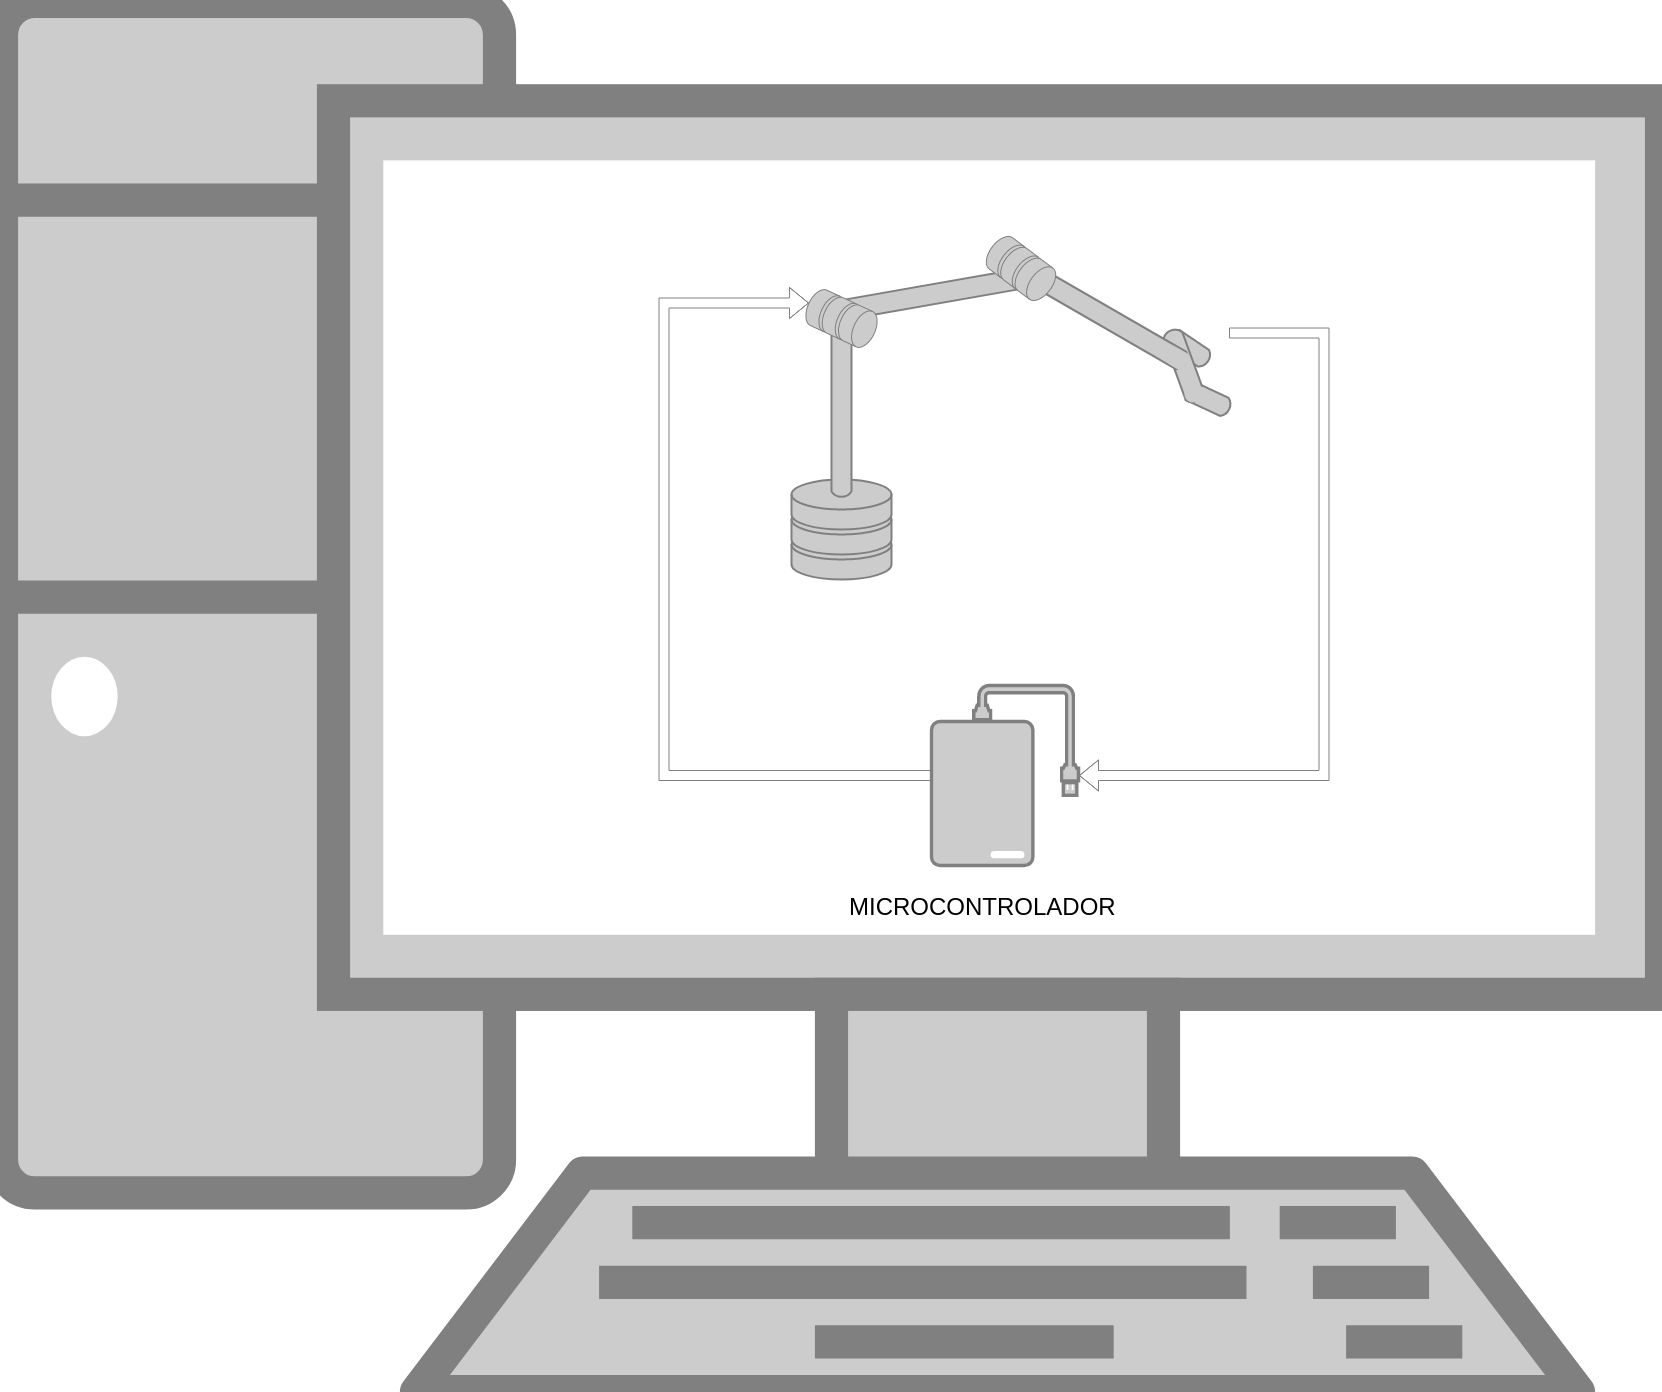
\includegraphics[width = 0.6\columnwidth]{Imagens/plantaSimulada.png}
    \caption{Planta e controlador simulados}
    \fonte{Do autor}
    \label{fig:plantaSimulada}
  \end{subfigure}%
  \begin{subfigure}{.5\textwidth}
    \centering
    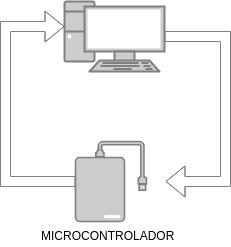
\includegraphics[width = 0.5\columnwidth]{Imagens/solucaoModelo.png}
    \caption{Solução para o modelo simulado da planta}
    \fonte{Do autor}
    \label{fig:solucaoModelo}
  \end{subfigure}%
  \\[5ex]
  \begin{subfigure}{\textwidth}
    \centering
    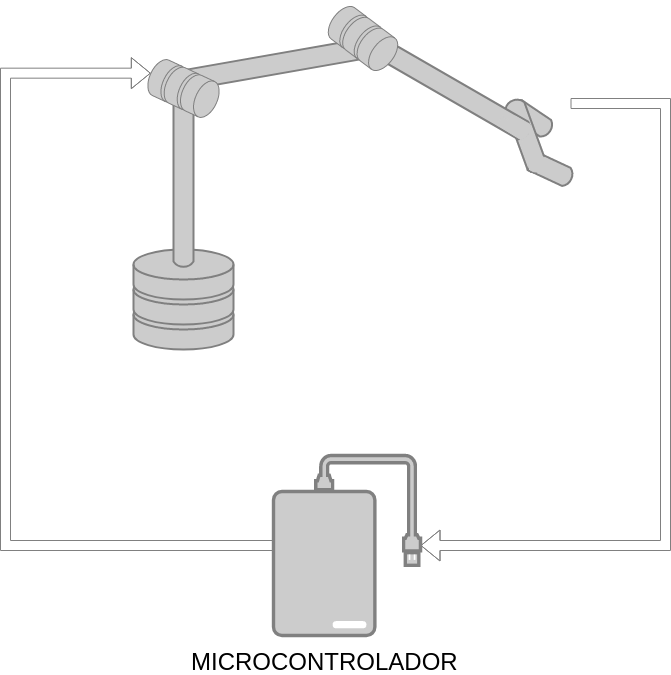
\includegraphics[width = 0.4\columnwidth]{Imagens/solucaoPlanta.png}
    \caption{Solução para a planta física}
    \fonte{Do autor}
    \label{fig:solucaoPlanta}
  \end{subfigure}%
  \caption{Diagramas das etapas da técnica \textit{Hardware-in-the-loop}}
  
  \label{fig:simulacoes} 

\end{figure}

\section{Resumo do Capítulo}
\markright{\thesection ~~~ Metodologia}
\label{metodo1b}

Este capítulo apresentou de forma sucinta a metodologia de projeto seguida para 
alcançar os objetivos propostos neste trabalho. No próximo capítulo são realizadas 
as modelagens cinemática e dinâmica do manipulador, a partir das quais o ambiente de 
simulação foi construído.


\clearpage